% !TeX root = ..//diffgeo_main.tex
\chapter{Differenzierbare Mannigfaltigkeiten}
\section*{Worum geht es in der Differentialgeometrie?}
Die zentralen Objekte der Differentialgeometrie sind Mannigfaltigkeiten. Das Ziel ist es, Analysis und Geometrie auf solchen Mannigfaltigkeiten zu betreiben. \\
Wir beginnen zunächst einmal mit einer kurzen Gegenüberstellung der bereits bekannten Konzepte aus dem $\mathbb{R}^n$ mit den korrespondierenden Begriffen der Differentialgeometrie, welche wir in den kommenden Vorlesungen noch genauer kennenlernen werden.

%Vergleich
\begin{figure}[H]
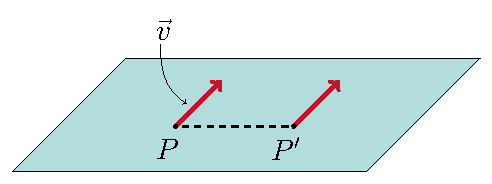
\includegraphics[scale=0.8]{figures/tikz/plane.pdf}
\hspace{2cm}
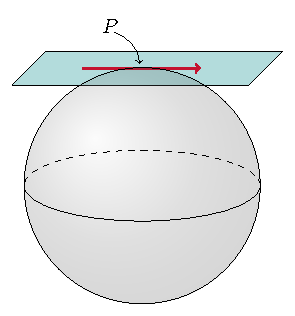
\includegraphics[scale=0.9]{figures/tikz/sphere_with_plane.pdf}
\end{figure}

\begin{figure}[H]
\centering
\begin{tabular}{>{\centering}p{.45\textwidth} | >{\centering}p{.45\textwidth}} 
$\mathbb{R}^n$ \vspace{5pt} & $\Huge\mathcal{M}$  \vspace{5pt} \tabularnewline \hline 
\vspace{5pt} Parallelverschiebung & \vspace{5pt} Begriff des Zusammenhangs\tabularnewline 
\vspace{5pt} Gerade = kürzeste Verbindung & \vspace{5pt} Konzept der Geodätischen \tabularnewline 
\vspace{5pt} flacher Raum & \vspace{5pt} gekrümmter Raum \tabularnewline 
\vspace{5pt} Skalarprodukt & \vspace{5pt} Riemannsche Metrik \tabularnewline 
\end{tabular}
\end{figure}
\section{Definitionen}
Um differenzierbare Mannigfaltigkeiten definieren zu können wiederholen wir zunächst die Definition eines topologischen Raumes. \\
\phantom{.}\\
\bfseries Erinnerung: \normalfont $M \subseteq \mathbb{R}^n$ offen, wenn $\forall p \in U \ \exists \ \varepsilon>0$, sodass $B_{\varepsilon}(p) \subset U$. Dieser Begriff von Offenheit heißt \textit{euklidische Topologie} \normalfont und erfüllt:
\begin{enumerate}
\item[i)] $\emptyset, \mathbb{R}^n$ offen
\item[ii)] $U, V \subset \mathbb{R}^n$ offen $\Rightarrow U \cap V$ offen in $\mathbb{R}^n$
\item [iii)] $U_i, i \in $ I offen in $\mathbb{R}^n \Rightarrow \bigcup\limits_{i \in \text{I}} U_i \subset \mathbb{R}^n$ offen
\end{enumerate} 


\begin{figure}[H]
\centering
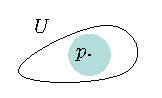
\includegraphics[scale=1.5]{figures/tikz/openset.pdf}
\caption{Offene Menge}
\label{img:offenemenge}
\end{figure} 

\begin{defs}[Topologischer Raum]
Ein topologischer Raum ist eine Menge $X$ zusammen mit einer Menge $\mathcal{O} \subset \mathcal{P}(X)$, sodass:
\begin{enumerate}
	\item[i)] $\emptyset, X \in \mathcal{O}$
	\item[ii)] $U, V \in \mathcal{O} \Rightarrow  U \cap V \in \mathcal{O}$
	\item [iii)] $U_i \in \mathcal{O} \Rightarrow\bigcup\limits_{i \in \text{I}} U_i \in \mathcal{O}$
\end{enumerate} 
\end{defs}
\begin{bsp}
\begin{enumerate}
	\item[a)] $( X, \mathcal{O} = \mathcal{P}(X) )$
	\item[b)] $N \subset X$ Teilmenge. Dann ist auch $(N,\mathcal{O}_1)$ ein topologischer Raum, wobei $\mathcal{O}_1$ wie folgt gegeben ist:\\
	\center{$V \in \mathcal{O}_1 \Leftrightarrow \ \exists \ U \in \mathcal{O}$, sodass $V= N \cap U$}
\end{enumerate}
%\begin{figure}[h]
%\centering
%\includegraphics[width=0.35\linewidth]{figures/scan/teilmengetopologie.png}
%\label{img:teilmengetopologie}
%\end{figure}
Teilmengen topologischer Räume sind topologische Räume.
\end{bsp}

\begin{defs}[Topologische Mannigfaltigkeiten]
Eine topologische Mannigfaltigkeit ist ein topologischer Raum $\mathcal{M}$ der Dimension $n$ mit folgenden Eigenschaften:
\begin{enumerate}
	\item[i)] $\mathcal{M}$ ist hausdorffsch. Das heißt $\forall \ p, q \in \mathcal{M}$ mit $p \neq q \  \exists$ \ zwei disjunkte, offene Umgebungen $U \ni p$ und $V \ni q$ wobei $U, V \in \mathcal{O}$
\begin{figure}[H]
\centering
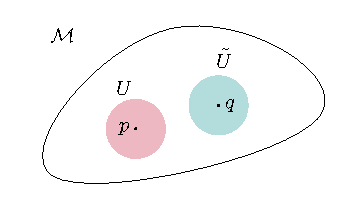
\includegraphics[width=0.4\linewidth]{figures/tikz/hausdorff.pdf}
\caption{Hausdorff'sche Eigenschaft}
\label{img:hausdorff}
\end{figure} 	
	\item[ii)] \textbf{2. Abzählbarkeitsaxiom}  \\
	$\mathcal{M}$ hat eine abzählbare Basis der Topologie, das heißt es existiert eine abzählbare Menge $\{U_1, \dots, U_k, \dots\}$ 
	offener Teilmengen oder abzählbar viele offene Mengen $U_1, \dots, U_k, \dots$ mit $U_i \in \mathcal{O}$, 
	sodass $\forall p \in \mathcal{M}$ und alle Umgebungen $U$ von $p$ gibt es ein $K$ sodass $p \in U_k \subseteq U$.
	\item [iii)] $\mathcal{M}$ ist homöomorph zu $\mathbb{R}^n$, das heißt $\forall p \in \mathcal{M}$ existiert eine Umgebung $U$ von $p$ und ein \bfseries Homöomorphismus \normalfont $X: U \rightarrow V \subseteq \mathbb{R}^n$ (offen).
\end{enumerate} 
\end{defs}
\begin{minipage}[H]{.8\textwidth}
\begin{defs}[Karte, Atlas]
	Das Paar $(X, U)$ heißt \textbf{Karte} von $\mathcal{M}$ um $p$. \\
	Eine Menge $\mathcal{A} = \{(x_{\alpha},U_{\alpha})_{\alpha \in \mathcal{A}}\}$ von Karten heißt \textbf{Atlas} von $\mathcal{M}$, falls \\
	\begin{align}
	\bigcup\limits_{\alpha \in \mathcal{A}} U_\alpha = \mathcal{M}
	\end{align}
\end{defs}
\end{minipage}
\hspace{1cm}
\begin{minipage}[H]{.2\textwidth}
\vspace{-0.5cm}
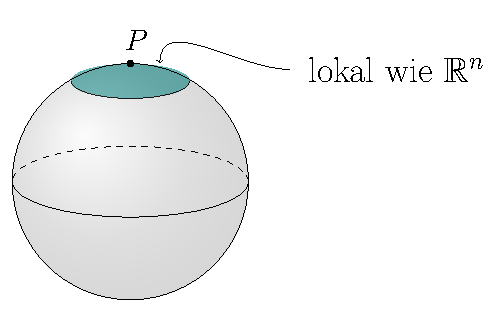
\includegraphics[scale=0.5]{figures/tikz/sphere_local_rn}
\end{minipage}


Topologische Mannigfaltigkeiten sind die Grundbausteine. Nun wollen wir auf diesen Mannigfaltigkeiten Geometrie betreiben. Dafür benötigen wir mehr Struktur. Wir wollen die differenzierbare Struktur des $\mathbb{R}^n$ auf unseren Mannigfaltigkeiten "holen".

\begin{defs}[Kartenwechsel]
Seien $x_{\alpha}$ und $x_{\beta}$ zwei Karten, dann ist der Kartenwechsel wie folgt definiert: \\
\begin{align}
x_{\alpha}\circ x_{\beta}^{-1}: x_{\beta}(U_{\alpha}\cap U_{\beta}) \rightarrow x_{\alpha}(U_{\alpha}\cap U_{\beta}) \subseteq \mathbb{R}^n
\end{align}
Dies ist ein Homöomorphismus.

\begin{figure}[H]
\centering
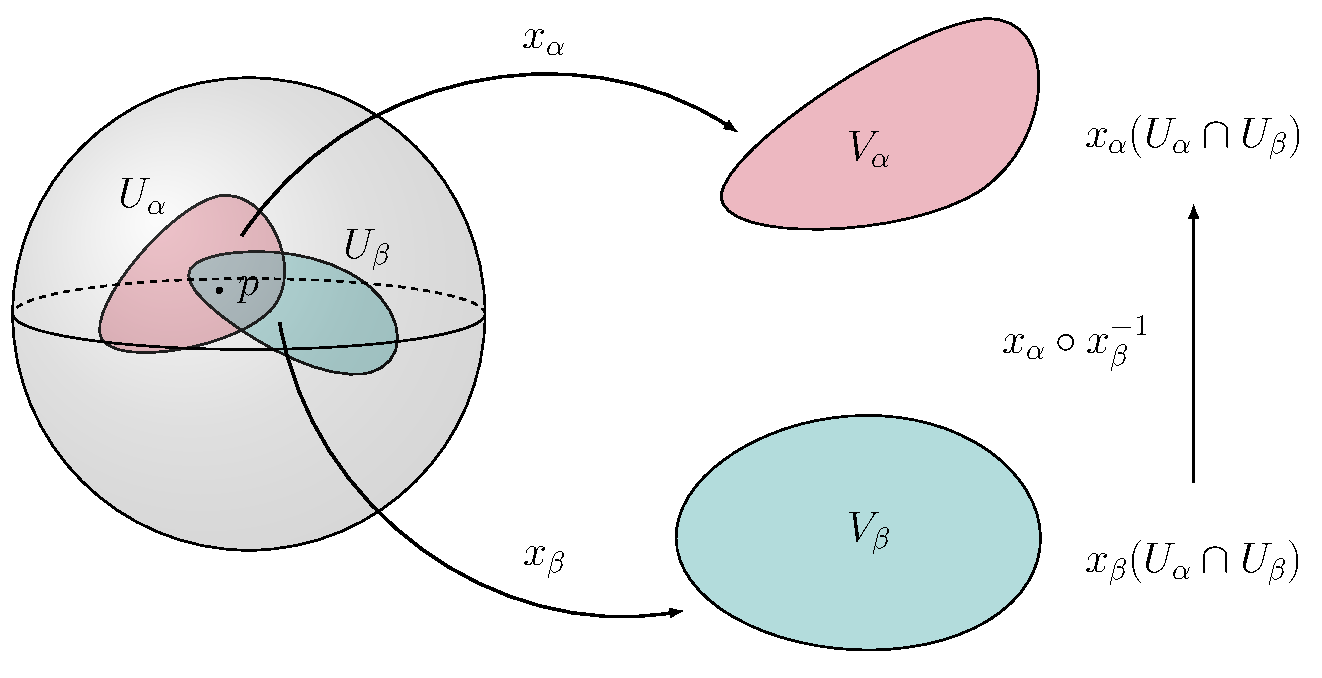
\includegraphics[width=1.0\linewidth]{figures/tikz/map_change.pdf}
\caption{Kartenwechsel}
\label{img:kartenwechsel}
\end{figure} 

\end{defs}
Nun wollen wir, dass $x_{\alpha}\circ x_{\beta}^{-1}$ Diffeomorphismen sind.
\begin{defs}
Sei $ \mathcal{M}$ eine topologische Mannigfaltigkeit.
\begin{enumerate}
	\item[a)] Ein Atlas $\mathcal{A} = \{(x_{\alpha},U_{\alpha})\}$ auf $\mathcal{M}$ heißt $C^{\infty}$-Atlas, falls alle Kartenwechsel $x_{\alpha}\circ x_{\beta}^{-1}$ mit $\alpha, \beta \in A \ C^{\infty}$-Diffeomorphismen sind.
	\item[b)] Sei $\mathcal{A}$ ein $C^{\infty}$-Atlas von $\mathcal{M}$. \\
	Eine Karte $(x,U)$ ist verträglich mit $\mathcal{A}$, falls $x \circ x_\alpha^{-1}$ ein $C^{\infty}$-Diffeomorphismus ist.
\end{enumerate}
\end{defs}
Gegeben ein $C^{\infty}$-Atlas, so kann man diesen zu einem \textit{maximalen} $C^{\infty}$-Atlas vervollständigen. Maximal bedeutet hierbei, dass der Atlas nicht strikt in einem anderen enthalten ist.

